\sectionframe{Recap}
\section{Recap}

\begin{frame}{Complex Model}
	\vspace{-1em}
	\begin{itemize}
		\item We started with a complex model describing the dynamics of a power converter
		\item It exhibits interesting dynamics we want to understand
		\item Chains of parameter regions with the same period, partially bistability-affected
		      %\item Parameter regions with 2 coexisting cycles in between parameter regions with single cycles
	\end{itemize}
	\vspace{-.5em}
	\begin{figure}
		\stackunder[5pt]{
			\includegraphics[width=0.3 \textwidth]{99_Yunus/2D_Period_Zoomed/result.png}
		}{2D period scan}
		\stackunder[5pt]{
			\includegraphics[width=0.3 \textwidth]{99_Yunus/Period12/Cobweb_A_12/result.png}
		}{Cobweb at point $A$}
		\stackunder[5pt]{
			\includegraphics[width=0.3 \textwidth]{99_Yunus/Period12/Cobweb_B2/result.png}
		}{Cobweb at point $B$}
	\end{figure}
\end{frame}

\begin{frame}{Original Model (1/3)}
	\vspace{-2.0em}
	\begin{align}
		\theta      & \mapsto  F(\theta) \mod 2 \pi
		\\
		F(\theta)   & = \begin{cases}
			                F_1(\theta) & \text{if } q \cdot \cos(\theta) > 0 \\
			                F_2(\theta) & \text{if } q \cdot \cos(\theta) < 0
		                \end{cases}
		\\
		F_1(\theta) & = \begin{cases}
			                \theta + z_{L_+} + z_1 & \text{if } z_{L_+} < z_{L_0} \\
			                \theta + z_{L_0} + z_2 & \text{if } z_{L_+} > z_{L_0}
		                \end{cases}
		\\
		F_2(\theta) & = \begin{cases}
			                \theta + z_{R_+} + z_3 & \text{if } z_{R_+} < z_{R_0} \\
			                \theta + z_{R_0} + z_4 & \text{if } z_{R_+} > z_{R_0}
		                \end{cases}
	\end{align}

	\pause
	\vspace{2em}
	This looks ok, but how are these values defined?
	\begin{align*}
		z_1, z_2, z_3, z_4, z_{L_+}, z_{L_-}, z_{R_+}, \text{ and } z_{R_0}
	\end{align*}
\end{frame}

\begin{frame}{Original Model (2/3)}
	\vspace{-1em}
	The smallest non-negative solutions to the following implicit equations
	\begin{subequations}
		\begin{align}
			(q \cdot \cos(\theta) + \mu \cdot \chi) \cdot e^{\lambda \cdot z_{L_+}}
			 & = q \cdot \cos(\theta + z_{L_+}) + \chi \\
			(q \cdot \cos(\theta) + \mu \cdot \chi) \cdot e^{\lambda \cdot z_{L_0}}
			 & = q \cdot \cos(\theta + z_{L_0}) - \chi \\
			(q \cdot \cos(\theta) - \mu \cdot \chi) \cdot e^{\lambda \cdot z_{R_+}}
			 & = q \cdot \cos(\theta + z_{R_+}) - \chi \\
			(q \cdot \cos(\theta) - \mu \cdot \chi) \cdot e^{\lambda \cdot z_{R_0}}
			 & = q \cdot \cos(\theta + z_{R_0}) + \chi
		\end{align}
	\end{subequations}
	\vspace{-2em}
	\begin{subequations}
		\begin{align}
			(q \cdot \cos(\theta + z_{L_+}) + \chi + 1) \cdot e^{\lambda \cdot z_1} - 1
			 & = q \cdot  \cos(\theta + z_{L_+} + z_1) + \mu \cdot \chi \\
			(q \cdot \cos(\theta + z_{L_0} + z_2) - \chi - 1) \cdot e^{\lambda \cdot z_2} + 1
			 & = q \cdot  \cos(\theta + z_{L_0} + z_2) - \mu \cdot \chi \\
			(q \cdot \cos(\theta + z_{R_+}) + \chi + 1) \cdot e^{\lambda \cdot z_3} - 1
			 & = q \cdot  \cos(\theta + z_{L_+} + z_1) + \mu \cdot \chi \\
			(q \cdot \cos(\theta + z_{R_0} + z_4) - \chi - 1) \cdot e^{\lambda \cdot z_4} + 1
			 & = q \cdot  \cos(\theta + z_{R_0} + z_2) - \mu \cdot \chi
		\end{align}
	\end{subequations}
	\begin{flushright}
		Definition from \cite{akyuz2022}
	\end{flushright}
\end{frame}

\begin{frame}{Approach}
	\vspace{-1em}
	Construct a simplified model with similar characteristics
	\pause
	\begin{itemize}
		\item Symmetry $F(\theta + \pi) = F(\theta) + \pi \mod 2\pi$ \hfill \cite{akyuz2022} \pause
		\item Branches $f_{\A}$ and $f_{\C}$ move up \pause
		\item The values at the left border of branches $f_{\B}$ and $f_{\D}$ move down \pause
		\item Model branches $f_\A$ and $f_\C$ quadratic \pause
		\item Model branches $f_\C$ and $f_\D$ simplified as linear
	\end{itemize}

	\begin{figure}
		\stackunder[5pt]{
			\includegraphics[width=0.2 \textwidth]{99_Yunus/ParameterEffects/E0/illustration.png}
		}{Effect of $E_0$}
		\stackunder[5pt]{
			\includegraphics[width=0.2 \textwidth]{99_Yunus/ParameterEffects/hi/illustration.png}
		}{Effect of $\chi_0$}
		\stackunder[5pt]{
			\includegraphics[width=0.2 \textwidth]{60_MinimalRepr/ParameterEffects/p_x/illustration.png}
		}{Effect of $p_x$}
		\stackunder[5pt]{
			\includegraphics[width=0.2 \textwidth]{60_MinimalRepr/ParameterEffects/p_y/illustration.png}
		}{Effect of $p_y$}
	\end{figure}
\end{frame}

\begin{frame}{Minimal Reproducing Model Dynamics}
	\vspace{-1em}
	\begin{figure}
		\stackunder[5pt]{
			\includegraphics[width=0.3 \textwidth]{99_Yunus/2D_Period_Zoomed/result.png}
		}{Original model}
		\qquad
		\stackunder[5pt]{
			\includegraphics[width=0.3 \textwidth]{60_MinimalRepr/2D_Period_Whole_noPoints/result.png}
		}{Simplified model}
	\end{figure}
	With this simplified model, we explained the structures
\end{frame}

\begin{frame}{Definition of the Minimal Reproducing Model (1/2)}
	\vspace{-3.0em}
	\begin{align}
		x \mapsto f(x) \mod 1
	\end{align}

	\begin{align}
		f(x) & = \begin{cases}
			         g(x)                                        & \text{ if } x < \frac{1}{2} \\
			         g\left(x - \frac{1}{2}\right) + \frac{1}{2} & \text{ else}
		         \end{cases}
	\end{align}

	\begin{align}
		g(x) & = \begin{cases}
			         l(x) = a_L \cdot x^2 + b_L \cdot x + c_L & \text{ if } x < \frac{1}{4} \\
			         r(x) = b_R \cdot x + c_R                 & \text{ else}
		         \end{cases}
	\end{align}
\end{frame}

\begin{frame}{Definition of the Minimal Reproducing Model (2/2)}
	\vspace{-1em}
	\begin{columns}
		\begin{column}{.7 \textwidth}
			Fixed parameters:
			\begin{align*}
				a_L = 4, b_L = -\frac{1}{2}
			\end{align*}

			Variable parameters
			\begin{align*}
				 & c_L, b_R, c_R                                                    \\
				\text{where} \qquad
				 & c_L = p_y,                                                       \\
				 & b_R = 4 \cdot (B - A), c_R = 2A - B                              \\
				\text {and} \qquad
				 & A = p_x, \text{and } B = \frac{1}{2} + \epsilon \text{ is fixed}
			\end{align*}

			$A$ and $B$ are intermediated parameters for modeling the values of the left ($A$) and right ($B$) borders of $r(x)$
		\end{column}
		\begin{column}{.3 \textwidth}
			\begin{figure}
				\centering
				\includegraphics[height=.5 \textheight]{60_MinimalRepr/ParameterEffects/AB/illustration.png}
				\caption*{Illustration of the parameters $A$ and $B$}
			\end{figure}
		\end{column}
	\end{columns}
\end{frame}

\begin{frame}{The Next Step}
	\vspace{-1em}
	Research questions:
	\begin{enumerate}
		\item Is there a simple model exhibiting the same behavior? \hfill \checkmark
		\item Was there something overlooked in the analysis of the original model? \hfill \checkmark
		      \pause
		\item What else can happen in the simplified model?
	\end{enumerate}

	\pause
	\vspace{1em}
	Hypothesis: Period Adding
	\begin{itemize}
		\item This is typical for models of power converters
		\item This is typical for piecewise increasing discontinuous models
		\item This is typical in between such chains of the same period
	\end{itemize}
\end{frame}

\begin{frame}{Symbolic Sequences}
	Cycles are described using symbolic sequences.
	Symbols indicate which branches the points of the cycle are on.
	\vspace{.5em}
	\begin{columns}
		\hspace{5em}
		\begin{column}{.3 \textwidth}
			\begin{figure}
				\includegraphics[width=\textwidth]{60_MinimalRepr/Cobweb_E16/result.png}
			\end{figure}
		\end{column}
		\hspace{3em}
		\begin{column}{.6 \textwidth}
			\begin{itemize}
				\item Cycle of period 16
				\item Symbolic Sequence: $\A^5\B^3\C^5\D^3$
			\end{itemize}
		\end{column}
	\end{columns}
\end{frame}
